\documentclass[a4paper,12pt]{article}
\usepackage[russian]{babel}
\usepackage[T2A]{fontenc}
\usepackage[utf8]{inputenc}
\usepackage{geometry}
\usepackage{amsmath}
\usepackage{graphicx}
\usepackage{cancel}
\usepackage{float} 
\usepackage{xcolor}
\usepackage{array}
\usepackage{caption}
\usepackage{booktabs}
\usepackage{amssymb}
\usepackage{subcaption}
\usepackage{pgfplots}
\pgfplotsset{compat=1.18}
\usetikzlibrary{arrows.meta, matrix}
\usepackage{capt-of}
\usepackage{multirow}
\usepackage[siunitx]{circuitikz}
\usepackage[bottom]{footmisc}
\usepackage{tcolorbox}
\usepackage{nicematrix}
\usepackage{tikz}
\usetikzlibrary{positioning, arrows.meta}

% --- hyperref ОДИН РАЗ ---
\usepackage{hyperref}
\hypersetup{linktoc=page}
\hypersetup{
	colorlinks=true,
	linkcolor=red,
	citecolor=red,
	urlcolor=red,
	filecolor=red,
}

% --- Содержание ---
\usepackage{tocloft}
\usepackage{etoolbox}
\usepackage{hyperref}
\hypersetup{
	colorlinks=true,
	linkcolor=red,
	citecolor=red,
	urlcolor=red,
}

% Патчим \tableofcontents: текст строк — без ссылок и чёрный
% Это делается через замену \contentsline внутри TOC
\preto\tableofcontents{%
	\begingroup
	% Переопределяем contentsline так, чтобы текст был чёрным без ссылки,
	% а номер страницы — красной ссылкой
	\renewcommand{\contentsline}[4]{%
		\ifnum\pdfstrcmp{##1}{section}=0
		\vskip 4pt{\normalfont\color{black}##2}\nobreak\hfill
		{\normalfont\color{red}\hyperlink{##4}{##3}}\par
		\else\ifnum\pdfstrcmp{##1}{subsection}=0
		\vskip 2pt\hspace{1.5em}{\normalfont\color{black}##2}\nobreak\hfill
		{\normalfont\color{red}\hyperlink{##4}{##3}}\par
		\else
		\vskip 1pt\hspace{3em}{\normalfont\color{black}##2}\nobreak\hfill
		{\normalfont\color{red}\hyperlink{##4}{##3}}\par
		\fi\fi
	}%
}
\appto\tableofcontents{\endgroup}

\newcommand{\figwidth}{0.7\textwidth}

% tocloft — только для отступов, без переопределения шрифтов
\usepackage{tocloft}

% --- Листинги ---
\usepackage{listings}

\definecolor{codebg}{RGB}{250,250,252}
\definecolor{linenumcolor}{RGB}{150,150,170}
\definecolor{mathblue}{RGB}{30,100,200}
\definecolor{mathorange}{RGB}{200,100,20}
\definecolor{matlabblue}{RGB}{0,0,200}
\definecolor{matlabgreen}{RGB}{30,130,30}
\definecolor{matlaborange}{RGB}{200,80,0}

\lstdefinelanguage{Mathematica}{
	keywords={Plot, Eigenvalues, MatrixExp, RiccatiSolve, IdentityMatrix,
		Inverse, Transpose, Simplify, Eigensystem, StateSpaceModel,
		ControllabilityMatrix, MatrixRank, Export, FileNameJoin,
		NotebookDirectory, ConstantArray, ZeroMatrix, NDSolve,
		Evaluate, LineLegend, Placed, Directive, Opacity, Filling,
		FillingStyle, PlotStyle, PlotLegends, PlotRange, Frame,
		Axes, FrameLabel, GridLines, GridLinesStyle, AspectRatio,
		Style, FontFamily, FontSize, Thick, Dashed, Dotted,
		DotDashed, RGBColor, GrayLevel, LegendLayout, LabelStyle,
		Subscript, Table, Do, Module, Block, If, True, False, Automatic},
	sensitive=true,
	morecomment=[s]{(*}{*)},
	morestring=[b]",
}

\lstdefinestyle{mma}{
	language=Mathematica,
	basicstyle=\ttfamily\small,
	keywordstyle=\color{mathblue}\bfseries,
	commentstyle=\color{linenumcolor}\itshape,
	stringstyle=\color{mathorange},
	numberstyle=\tiny\color{linenumcolor},
	numbers=left,
	numbersep=10pt,
	backgroundcolor=\color{codebg},
	frame=single,
	frameround=tttt,
	framesep=4pt,
	rulecolor=\color{mathblue!40},
	breaklines=true,
	tabsize=4,
	showstringspaces=false,
	captionpos=b,
	xleftmargin=15pt,
	xrightmargin=5pt,
}

\lstdefinestyle{matlab}{
	language=Matlab,
	basicstyle=\ttfamily\small,
	keywordstyle=\color{matlabblue}\bfseries,
	commentstyle=\color{matlabgreen}\itshape,
	stringstyle=\color{matlaborange},
	numberstyle=\tiny\color{linenumcolor},
	numbers=left,
	numbersep=10pt,
	backgroundcolor=\color{codebg},
	frame=single,
	frameround=tttt,
	framesep=4pt,
	rulecolor=\color{matlabblue!30},
	breaklines=true,
	tabsize=4,
	showstringspaces=false,
	captionpos=b,
	xleftmargin=15pt,
	xrightmargin=5pt,
	escapeinside={\%*}{*)},
	morekeywords={cvx_begin,cvx_end,sdp,variable,minimize,maximize},
}

\lstset{style=mma}

\renewcommand{\lstlistingname}{Листинг}
\DeclareCaptionFormat{redlisting}{#1\textcolor{red}{#2}#3}
\captionsetup[lstlisting]{format=redlisting}

\geometry{left=1.5cm, right=2cm, bottom=2cm, top=2cm}
\captionsetup[figure]{name=Рисунок}
\captionsetup[table]{name=Таблица}
\captionsetup{labelsep=endash}


\begin{document}
	
	\begin{titlepage}
		\centering
		
		\vspace*{0.5cm}
		{\small
			Министерство науки и высшего образования Российской Федерации\\[2pt]
			Федеральное государственное автономное образовательное учреждение\\
			высшего образования\\[2pt]
			\textbf{«Национальный исследовательский университет ИТМО»}\\
		}
		
		\vspace{0.8cm}
		\hrule height 0.8pt
		\vspace{0.3cm}
		
		{\large Факультет систем управления и робототехники}
		
		\vspace{0.3cm}
		\hrule height 0.4pt
		\vspace{2.5cm}
		
		{\Huge\bfseries ОТЧЁТ}\\[0.4cm]
		{\LARGE\bfseries о лабораторной работе №6}\\[0.8cm]
		
		\begin{tcolorbox}[
			colback=gray!4,
			colframe=gray!10,
			boxrule=0.8pt,
			arc=4pt,
			left=12pt, right=12pt, top=8pt, bottom=8pt
			]
			\centering
			{\large По дисциплине:\\[4pt]}
			{\large\bfseries «Адаптивное и робастное управление»}\\[10pt]
			{\large Тема:\\[4pt]}
			{\large\bfseries «Синтез адаптивного наблюдателя состояния линейного объекта»} \\[10pt]
			{\large Вариант: 8}
		\end{tcolorbox}
		\vspace{3cm}
		
		
		\begin{minipage}{0.45\textwidth}
			\raggedright
			{\large\bfseries Студенты:}\\[4pt]
			\textit{М.\,А.~Шульпин}\\
			\textit{Е.\,Д.~Охрименко}
		\end{minipage}%
		\hfill
		\begin{minipage}{0.45\textwidth}
			\raggedleft
			{\large\bfseries Преподаватель:}\\[4pt]
			\textit{Университет ИТМО, доцент \hfill А.\,В.~Парамонов}
		\end{minipage}
		
		\vfill
		\vspace{0.4cm}
		{\large Санкт-Петербург, 2026}
	\end{titlepage}
	
	\newpage
	\tableofcontents
	
	
\newpage
\section{Общие сведения и исходные данные}

\subsection{Математическая модель объекта управления}
Рассмотрим асимптотически устойчивый линейный объект управления во фробениусовой форме:
\begin{equation}
	\dot{x} = Ax + bu \qquad y = Cx
	\label{eq:obj_lab6}
\end{equation}
где:

\begin{enumerate}
	\item $x \in \mathbb{R}^2$ --- вектор состояния, недоступный прямому измерению;
	\item $u \in \mathbb{R}$ --- входной сигнал;
	\item $y \in \mathbb{R}$ --- выходной сигнал.
\end{enumerate}

Согласно нашему варианту возьмем коэффициенты передаточной функции объекта: 
\[a_1 = 3 \qquad  a_0 = 2 \qquad b_1 = 1 \qquad b_0 = 9\]
Матрицы объекта в канонической наблюдаемой форме форме:
\begin{equation}
	A = \begin{bmatrix} -a_1 & 1 \\ -a_0 & 0 \end{bmatrix} = \begin{bmatrix} -3 & 1 \\ -2 & 0 \end{bmatrix} \qquad 
	b = \begin{bmatrix} b_1 \\ b_0 \end{bmatrix} = \begin{bmatrix} 1 \\ 9 \end{bmatrix} \qquad 
	C = \begin{bmatrix} 1 & 0 \end{bmatrix}
\end{equation}
Спеткр матрицы $A$: $\sigma(A) = \{-1, -2\}$, объект асимптотически устойчив в разомкнутом состоянии. 

\subsection{Параметризация модели объекта}
Для синтеза адаптивного наблюдателя используем способ параметризации вектора состояния. Введем гурвицеву матрицу фильтров $A_0$, характеристический полином которой задается коэффициентами $k_1 = \sqrt{0{,}32}$ и $k_0 = 0{,}16$:
\begin{equation}
	A_0 = \begin{bmatrix} -k_1 & 1 \\ -k_0 & 0 \end{bmatrix} = \begin{bmatrix} -\sqrt{0{,}32} & 1 \\ -0{,}16 & 0 \end{bmatrix}
\end{equation}
Спектр матрицы $A_0$ лежит в левой комплексной полуплоскости.

На основе операторного метода вектор состояния $x(t)$ представляется в виде суммы:
\begin{equation}
	x = \sum_{i=1}^{2} (sI - A_0)^{-1} e_{3-i} [-(a_{i-1} - k_{i-1}) y] + \sum_{j=0}^{1} (sI - A_0)^{-1} e_{2-j} [b_j u]
	\label{eq:param_x}
\end{equation}
где $e_1 = \begin{bmatrix} 1 & 0 \end{bmatrix}^T$, $e_2 = \begin{bmatrix} 0 & 1 \end{bmatrix}^T$ --- единичные векторы. 

Выражение (\ref{eq:param_x}) можно переписать в компактной векторно-матричной форме:
\begin{equation}
	x = \xi \theta
	\label{eq:x_xi_theta}
\end{equation}
где $\xi \in \mathbb{R}^{2 \times 4}$ --- матрица, составленная из векторов состояний вспомогательных фильтров:
\begin{equation}
	\xi = \begin{bmatrix} \xi_{y0} & \xi_{y1} & \xi_{u0} & \xi_{u1} \end{bmatrix}
\end{equation}
а $\theta \in \mathbb{R}^4$ --- истинный вектор неизвестных параметров объекта:
\begin{equation}
	\theta = \begin{bmatrix} k_0 - a_0 \\ k_1 - a_1 \\ b_0 \\ b_1 \end{bmatrix} = \begin{bmatrix} 0{,}16 - 2 \\ \sqrt{0{,}32} - 3 \\ 9 \\ 1 \end{bmatrix} \approx \begin{bmatrix} -1{,}84 \\ -2{,}434 \\ 9 \\ 1 \end{bmatrix}
	\label{eq:theta_true_lab6}
\end{equation}
Значение (\ref{eq:theta_true_lab6}) используется при анализе параметрической ошибки:

\begin{equation}
	\tilde{\theta}(t) = \hat \theta - \theta
	\label{eq:bar_theta}
\end{equation}


Аналогичным образом параметризуется выходная переменная объекта. Поскольку:

\[y = x_1 = C x\] 


Запишем:
\begin{equation}
	y = C \xi \theta = \omega^T \theta
	\label{eq:y_omega_theta}
\end{equation}
где $\omega = \xi^T C^T \in \mathbb{R}^4$ --- вектор регрессора, состоящий из первых компонент векторов состояний фильтров:
\begin{equation}
	\omega = \begin{bmatrix} \xi_{y2, 1} & \xi_{y1, 1} & \xi_{u2, 1} & \xi_{u1, 1} \end{bmatrix}^T
\end{equation}

\subsection{Синтез адаптивного наблюдателя состояния}
Целью работы является построение оценки вектора состояния $\hat{x}(t)$ такой, что:

\[\lim_{t\to\infty} \|x(t) - \hat{x}(t)\| = 0\] 
при одновременной оценке неизвестного вектора параметров $\theta$.

Заменив в (\ref{eq:y_omega_theta}) истинные параметры $\theta$ на их оценки $\hat{\theta}$, получим настраиваемую модель выхода:
\begin{equation}
	\hat{y} = \omega^T \hat{\theta}
	\label{eq:y_hat}
\end{equation}
Введем ошибку идентификации выхода $\varepsilon = y - \hat{y}$. С учетом (\ref{eq:y_omega_theta}) и (\ref{eq:y_hat}) ошибка принимает вид стандартной статической модели:
\begin{equation}
	\varepsilon = \omega^T (\theta - \hat{\theta}) = \omega^T \tilde{\theta}
	\label{eq:epsilon}
\end{equation}
где $\tilde{\theta}$ --- вектор параметрических ошибок (\ref{eq:bar_theta}).

Для настройки оценок $\hat{\theta}$ выберем функцию Ляпунова: 

\[V = \frac{1}{2\gamma} \tilde{\theta}^T \tilde{\theta}\]

 Вычисление её производной дает алгоритм адаптации:
\begin{equation}
	\dot{\hat{\theta}} = \gamma \omega \varepsilon \qquad \hat{\theta}(0) = \mathbf{0}_{4 \times 1}
	\label{eq:adapt_law}
\end{equation}
где $\gamma > 0$ --- коэффициент адаптации, выбираемый экспериментальным путем. При таком выборе $\dot{V} = -\varepsilon^2 \leq 0$, что гарантирует ограниченность сигналов и асимптотическое стремление $\varepsilon$ к нулю.

Оценка вектора состояния $\hat{x}$ формируется на основе текущих оценок параметров и состояний фильтров:
\begin{equation}
	\hat{x} = \xi \hat{\theta} = \hat{\theta}_1 \xi_{y2} + \hat{\theta}_2 \xi_{y1} + \hat{\theta}_3 \xi_{u2} + \hat{\theta}_4 \xi_{u1}
	\label{eq:x_hat}
\end{equation}


\newpage
\section{Структурная схема системы в среде Simulink}


Смоделируем асимптотически устойчивый линейный объект управления в канонической форме:


\begin{figure}[H]
	\centering
	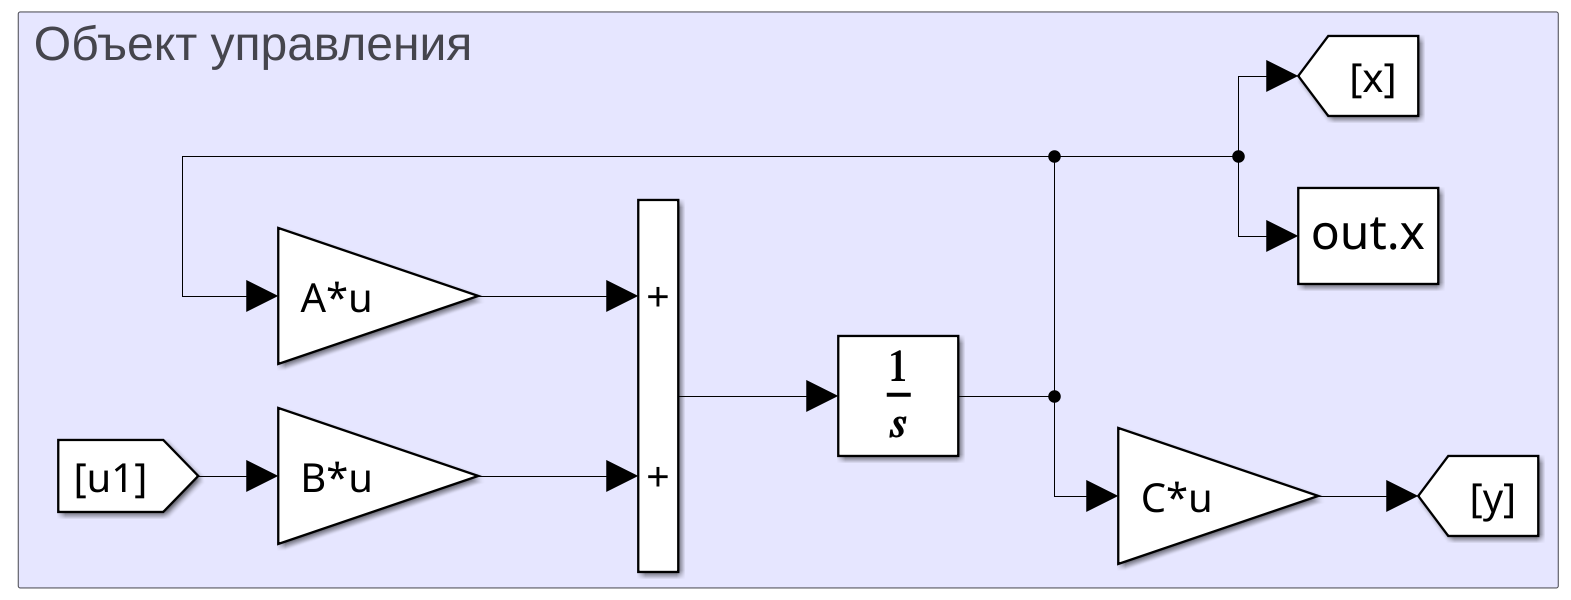
\includegraphics[width=0.7\textwidth]{../images/sim/obj.png}
	\caption{Объект управления}
	\label{fig:sim_obj}
\end{figure}

Для параметризации модели объекта используются вспомогательные фильтры с гурвицевой матрицей $A_0$. Выходы четырех фильтров (два по выходу $y$, два по входу $u$) объединяются в единый расширенный вектор состояний $\xi \in \mathbb{R}^{8 \times 1}$:
\begin{equation}
	\xi = \begin{bmatrix} Y_0 \\ Y_1 \\ U_0 \\ U_1 \end{bmatrix}
\end{equation}
где каждый компонент является вектором размерности $2 \times 1$.

\begin{figure}[H]
	\centering
	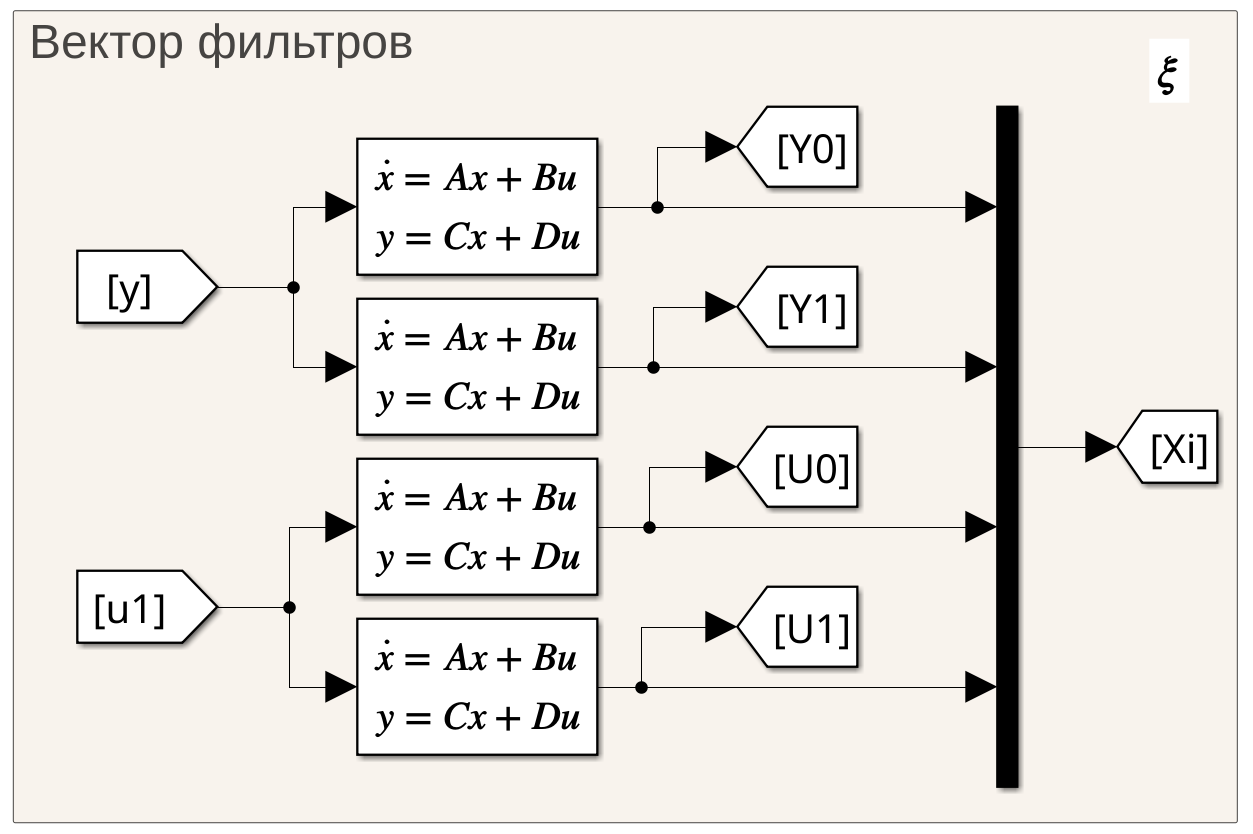
\includegraphics[width=0.55\textwidth]{../images/sim/xi.png}
	\caption{Формирование расширенного вектора состояний фильтров $\xi$}
	\label{fig:sim_xi}
\end{figure}

Вектор регрессора $\omega$ (вектор измеряемых функций) формируется путем выбора первых компонент из вектора $\xi$ с помощью вспомогательной $C_\xi$, которая извекает первые компоненты:
\begin{equation}
	\omega = C_\xi \xi, \quad C_\xi = \begin{bmatrix} 1 & 0 & 0 & 0 & 0 & 0 & 0 & 0 \\ 0 & 0 & 1 & 0 & 0 & 0 & 0 & 0 \\ 0 & 0 & 0 & 0 & 1 & 0 & 0 & 0 \\ 0 & 0 & 0 & 0 & 0 & 0 & 1 & 0 \end{bmatrix}
\end{equation}

\begin{figure}[H]
	\centering
	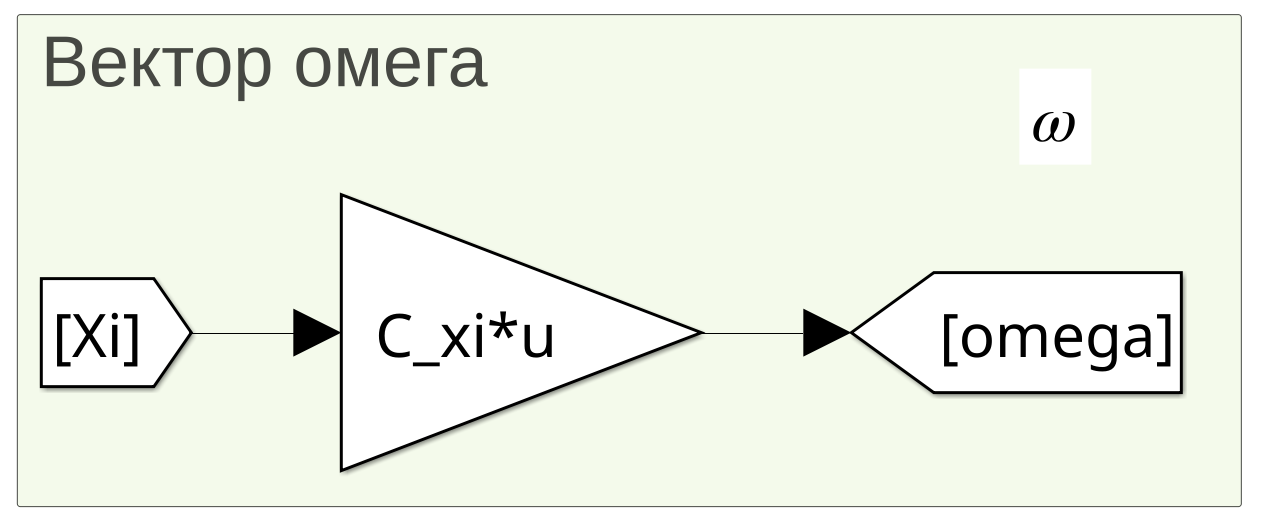
\includegraphics[width=0.4\textwidth]{../images/sim/omega.png}
	\caption{Формирование вектора регрессора $\omega$}
	\label{fig:sim_omega}
\end{figure}

Оценка выходной переменной формируется как скалярное произведение вектора оценок параметров $\hat{\theta}$ на вектор регрессора $\omega$:
\begin{equation}
	\hat{y} = \omega^T \hat{\theta}
\end{equation}

\begin{figure}[H]
	\centering
	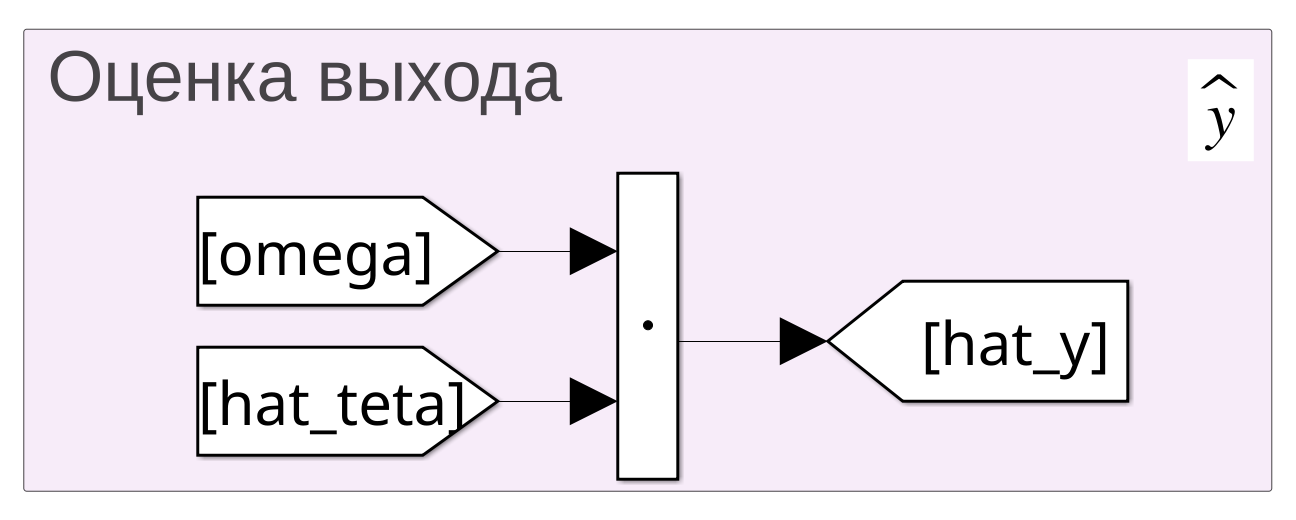
\includegraphics[width=0.4\textwidth]{../images/sim/hat_y.png}
	\caption{Блок формирования оценки выхода $\hat{y}$}
	\label{fig:sim_hat_y}
\end{figure}

Ошибка идентификации выхода вычисляется как разность между реальным и оцененным выходом:
\begin{equation}
	\varepsilon = y - \hat{y} = \omega^T \tilde{\theta}
\end{equation}

\begin{figure}[H]
	\centering
	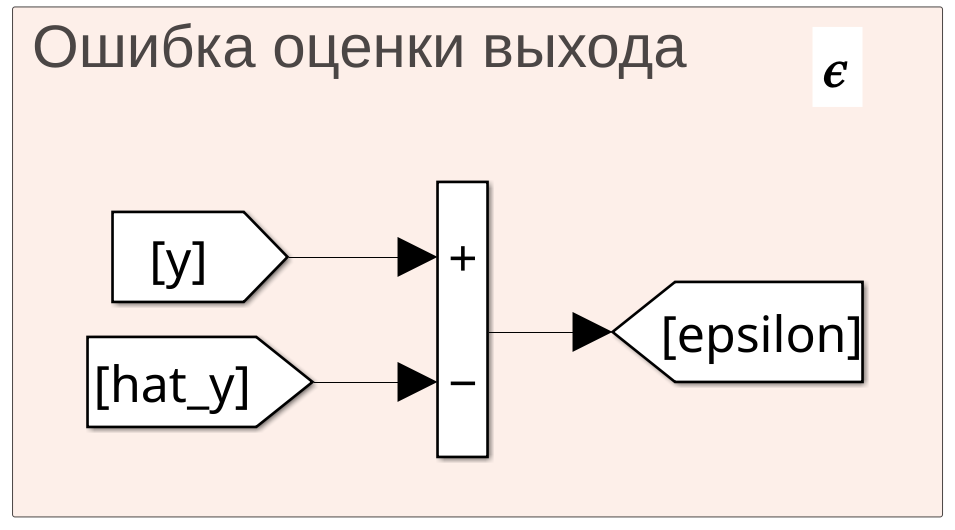
\includegraphics[width=0.35\textwidth]{../images/sim/epsilon.png}
	\caption{Блок вычисления ошибки идентификации $\varepsilon$}
	\label{fig:sim_epsilon}
\end{figure}

Для настройки оценок параметров используется градиентный алгоритм адаптации, синтезированный на основе функции Ляпунова:
\begin{equation}
	\dot{\hat{\theta}} = \gamma \omega \varepsilon, \qquad \hat{\theta}(0) = \mathbf{0}_{4 \times 1}
\end{equation}
где $\gamma > 0$ --- коэффициент адаптации.

\begin{figure}[H]
	\centering
	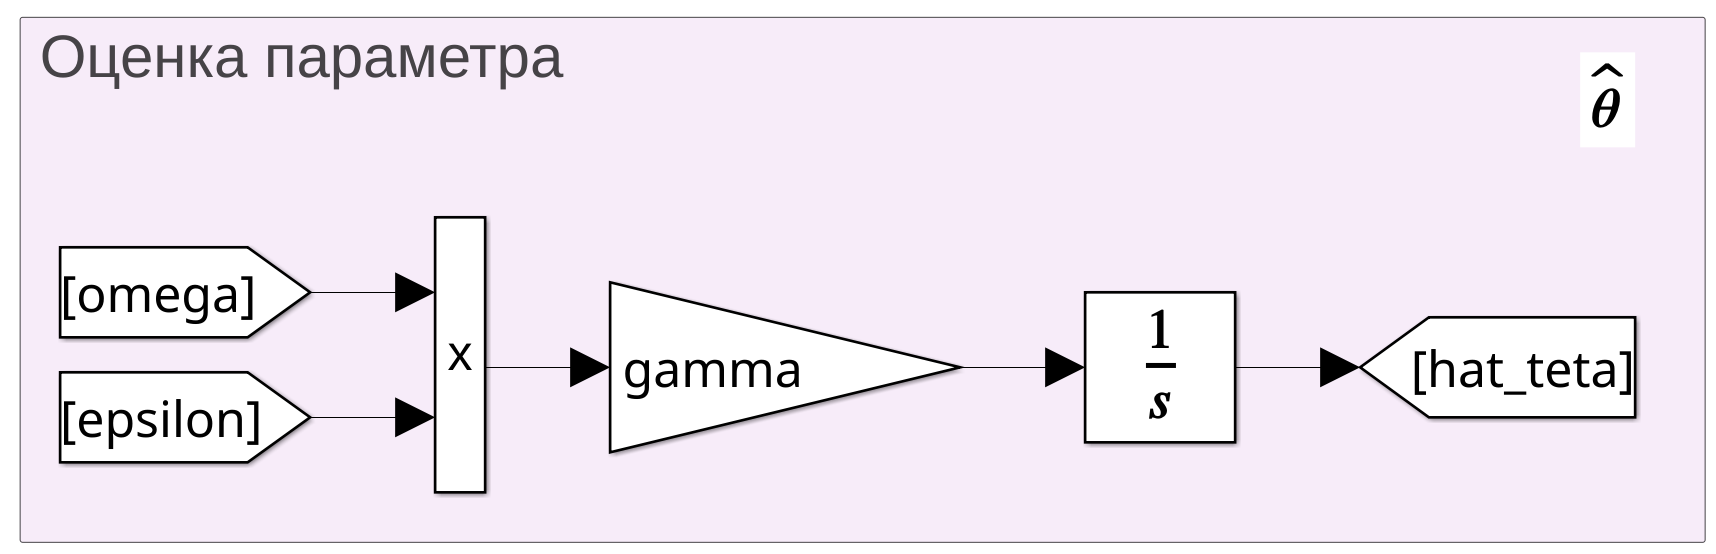
\includegraphics[width=0.6\textwidth]{../images/sim/hat_teta.png}
	\caption{Реализация алгоритма адаптации параметров}
	\label{fig:sim_hat_teta}
\end{figure}

Оценка вектора состояния объекта формируется на основе текущих оценок параметров и состояний фильтров. В матричном виде это записывается как:
\begin{equation}
	\hat{x} = \hat{\theta}_1 Y_0 + \hat{\theta}_2 Y_1 + \hat{\theta}_3 U_0 + \hat{\theta}_4 U_1
\end{equation}


\begin{figure}[H]
	\centering
	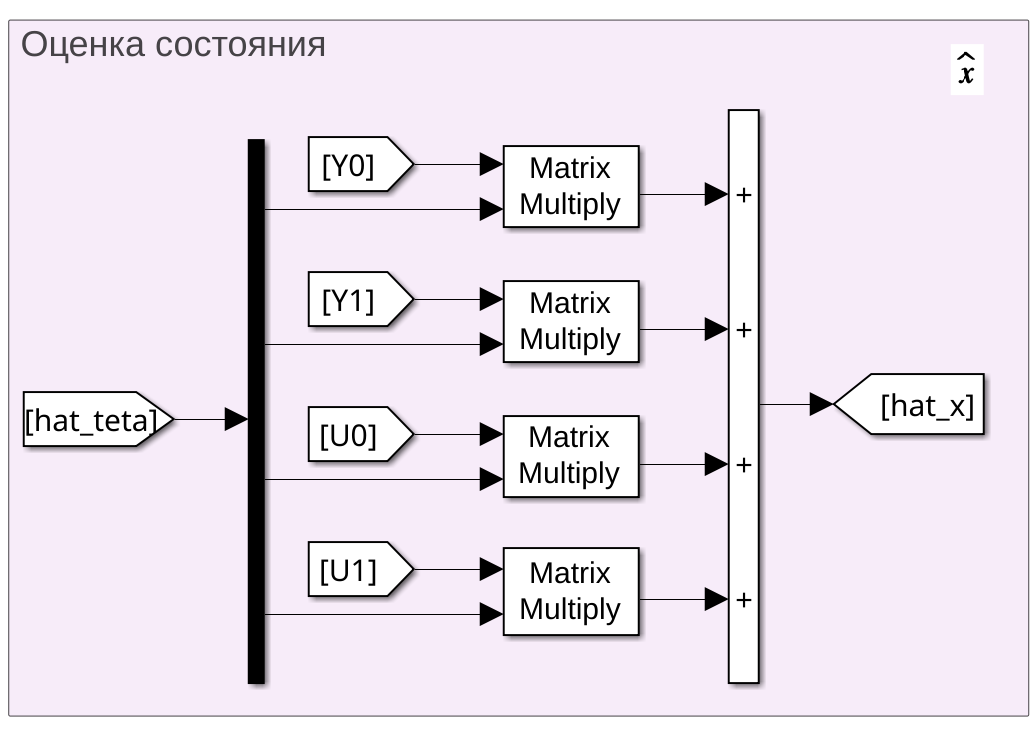
\includegraphics[width=0.7\textwidth]{../images/sim/hat_x.png}
	\caption{Формирование оценки вектора состояния $\hat{x}$}
	\label{fig:sim_hat_x}
\end{figure}


\newpage

\section{Результаты моделирования}

Моделирование проводилось при времени остановки $T = 50$~с и коэффициенте адаптации $\gamma = 0.005$.

\subsection{Одногармонический вход}
При подаче сигнала $u_1(t)=10\sin t$ условие неисчезающего возбуждения для 4-мерного регрессора не выполняется. Наблюдатель не способен восстановить состояние: ошибка $|x-\hat x|$ не стремится к нулю.

\begin{figure}[H]
	\centering
	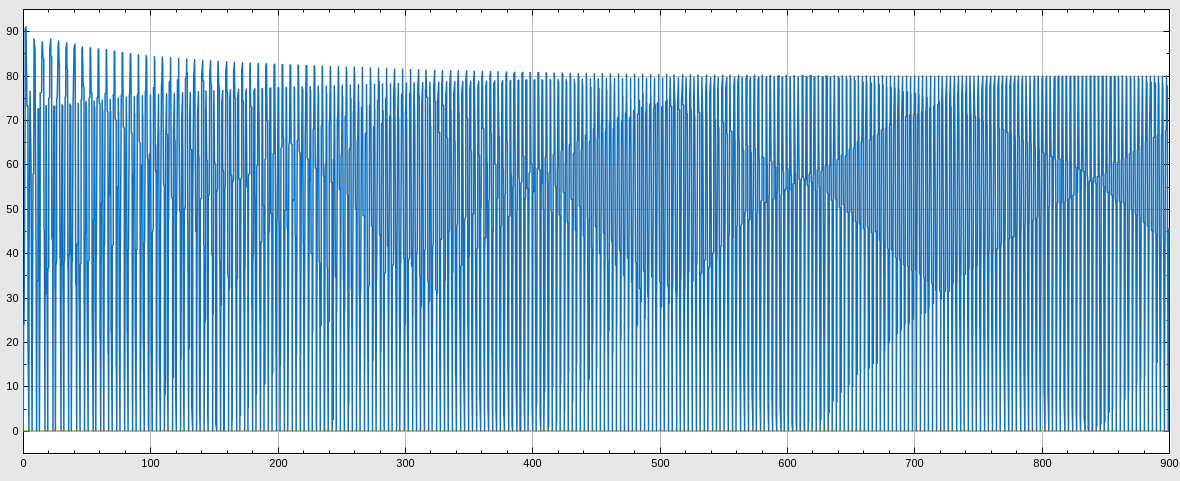
\includegraphics[width=1\textwidth]{../images/task1/u1_abs.png}
	\caption{Модуль ошибки $|x-\hat x|$ при $u_1(t)$, $\gamma=500$}
	\label{fig:res_u1_abs}
\end{figure}

\begin{figure}[H]
	\centering
	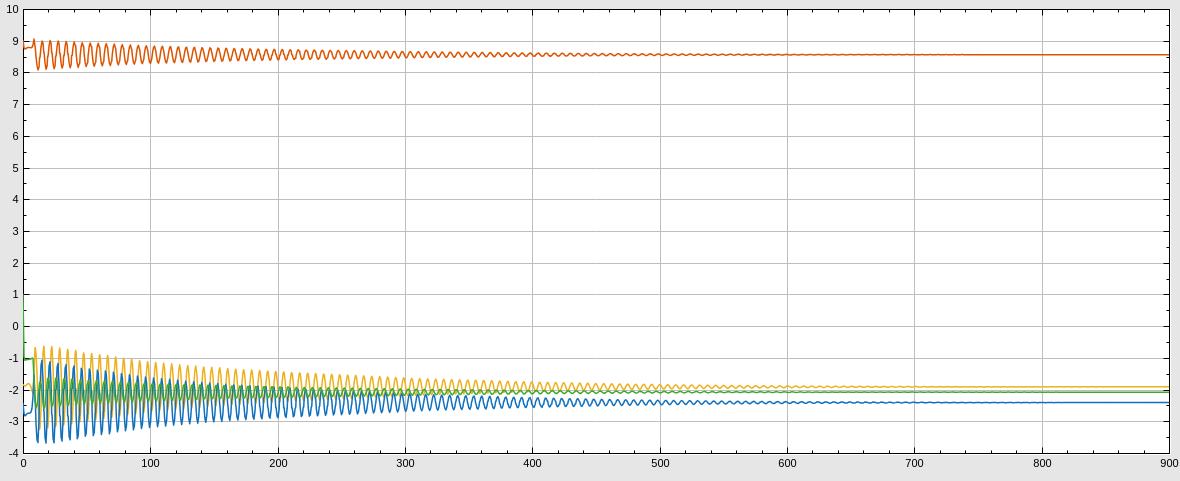
\includegraphics[width=1\textwidth]{../images/task1/u1_teta.png}
	\caption{Параметрические ошибки $\tilde\theta(t)$ при $u_1(t)$, $\gamma=500$}
	\label{fig:res_u1_teta}
\end{figure}

\subsection{Полигармонический вход}
При подаче сигнала $u_2(t) = 10\sin t + 5\cos 2t + 4\cos 4t + 3\cos 8t$ условие НВ выполняется. 


\begin{figure}[H]
	\centering
	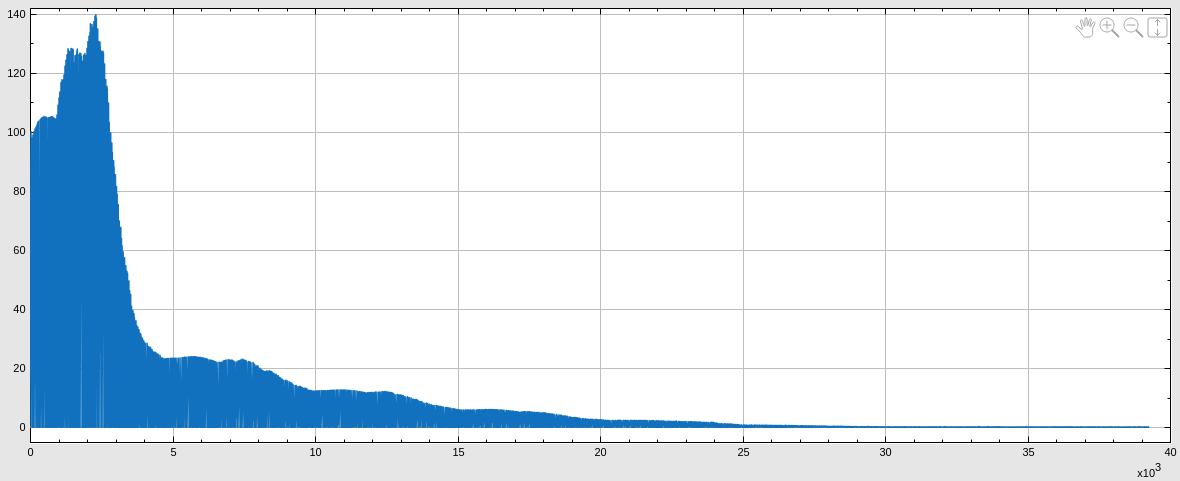
\includegraphics[width=1\textwidth]{../images/task2/u2_abs.png}
	\caption{Модуль ошибки $|x-\hat x|$ при $u_2(t)$, $\gamma=500$}
	\label{fig:res_u2_abs}
\end{figure}

\begin{figure}[H]
	\centering
	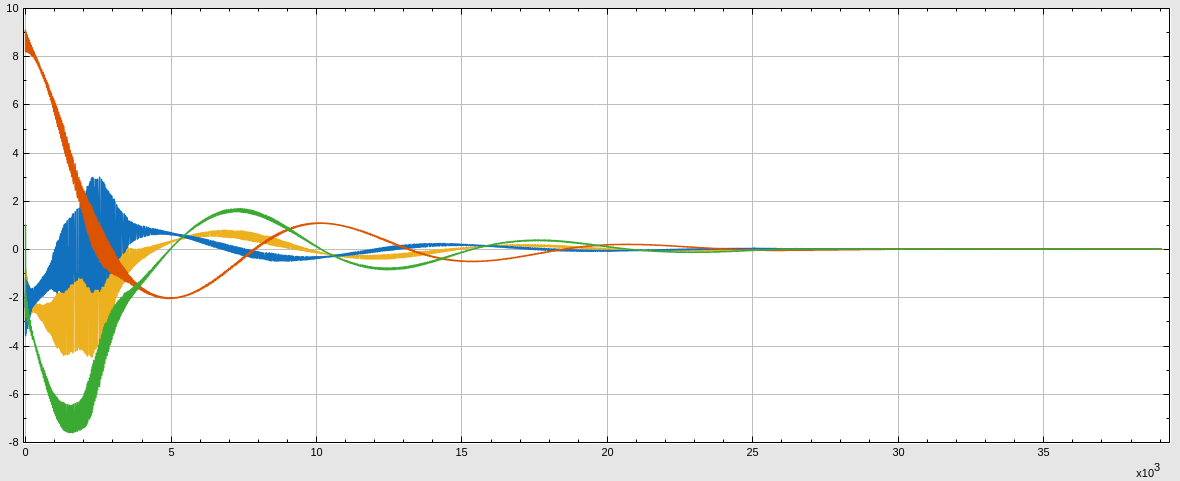
\includegraphics[width=1\textwidth]{../images/task2/u2_teta.png}
	\caption{Параметрические ошибки $\tilde\theta(t)$ при $u_2(t)$, $\gamma=500$}
	\label{fig:res_u2_teta}
\end{figure}


\newpage
\section{Выводы}
В ходе работы синтезирован адаптивный наблюдатель состояния для объекта 2-го порядка на основе параметризации вектора состояния. 

При соблюдении условия неисчезающего возбуждения ошибки параметров и слежеия стремятся к нулю экспоненциально.

	
\end{document}